\chapter{System Design and Architecture}
\label{chap:architecture}

This chapter provides a detailed technical blueprint of the TEKUTOKO platform. It outlines the high-level architectural paradigm, describes the individual components and their interactions, details the database schema, specifies the API design, and discusses the strategies employed to ensure system security, scalability, and maintainability.

\section{High-Level System Architecture}
\label{sec:arch-high-level}
The TEKUTOKO platform is engineered using a \textbf{microservice-based architecture} to promote modularity, independent scalability, and technological flexibility. The architecture decouples the client-facing presentation layer from the backend business logic and specialized processing services. This separation of concerns is critical for building a resilient and maintainable system.

The main components are the React frontend, a core Node.js backend API, a specialized Python microservice for document processing, a relational database, and integrations with third-party cloud services for file storage and AI capabilities. The overall architecture is depicted in Figure \ref{fig:system-architecture}.

\begin{figure}[htbp]
\centering
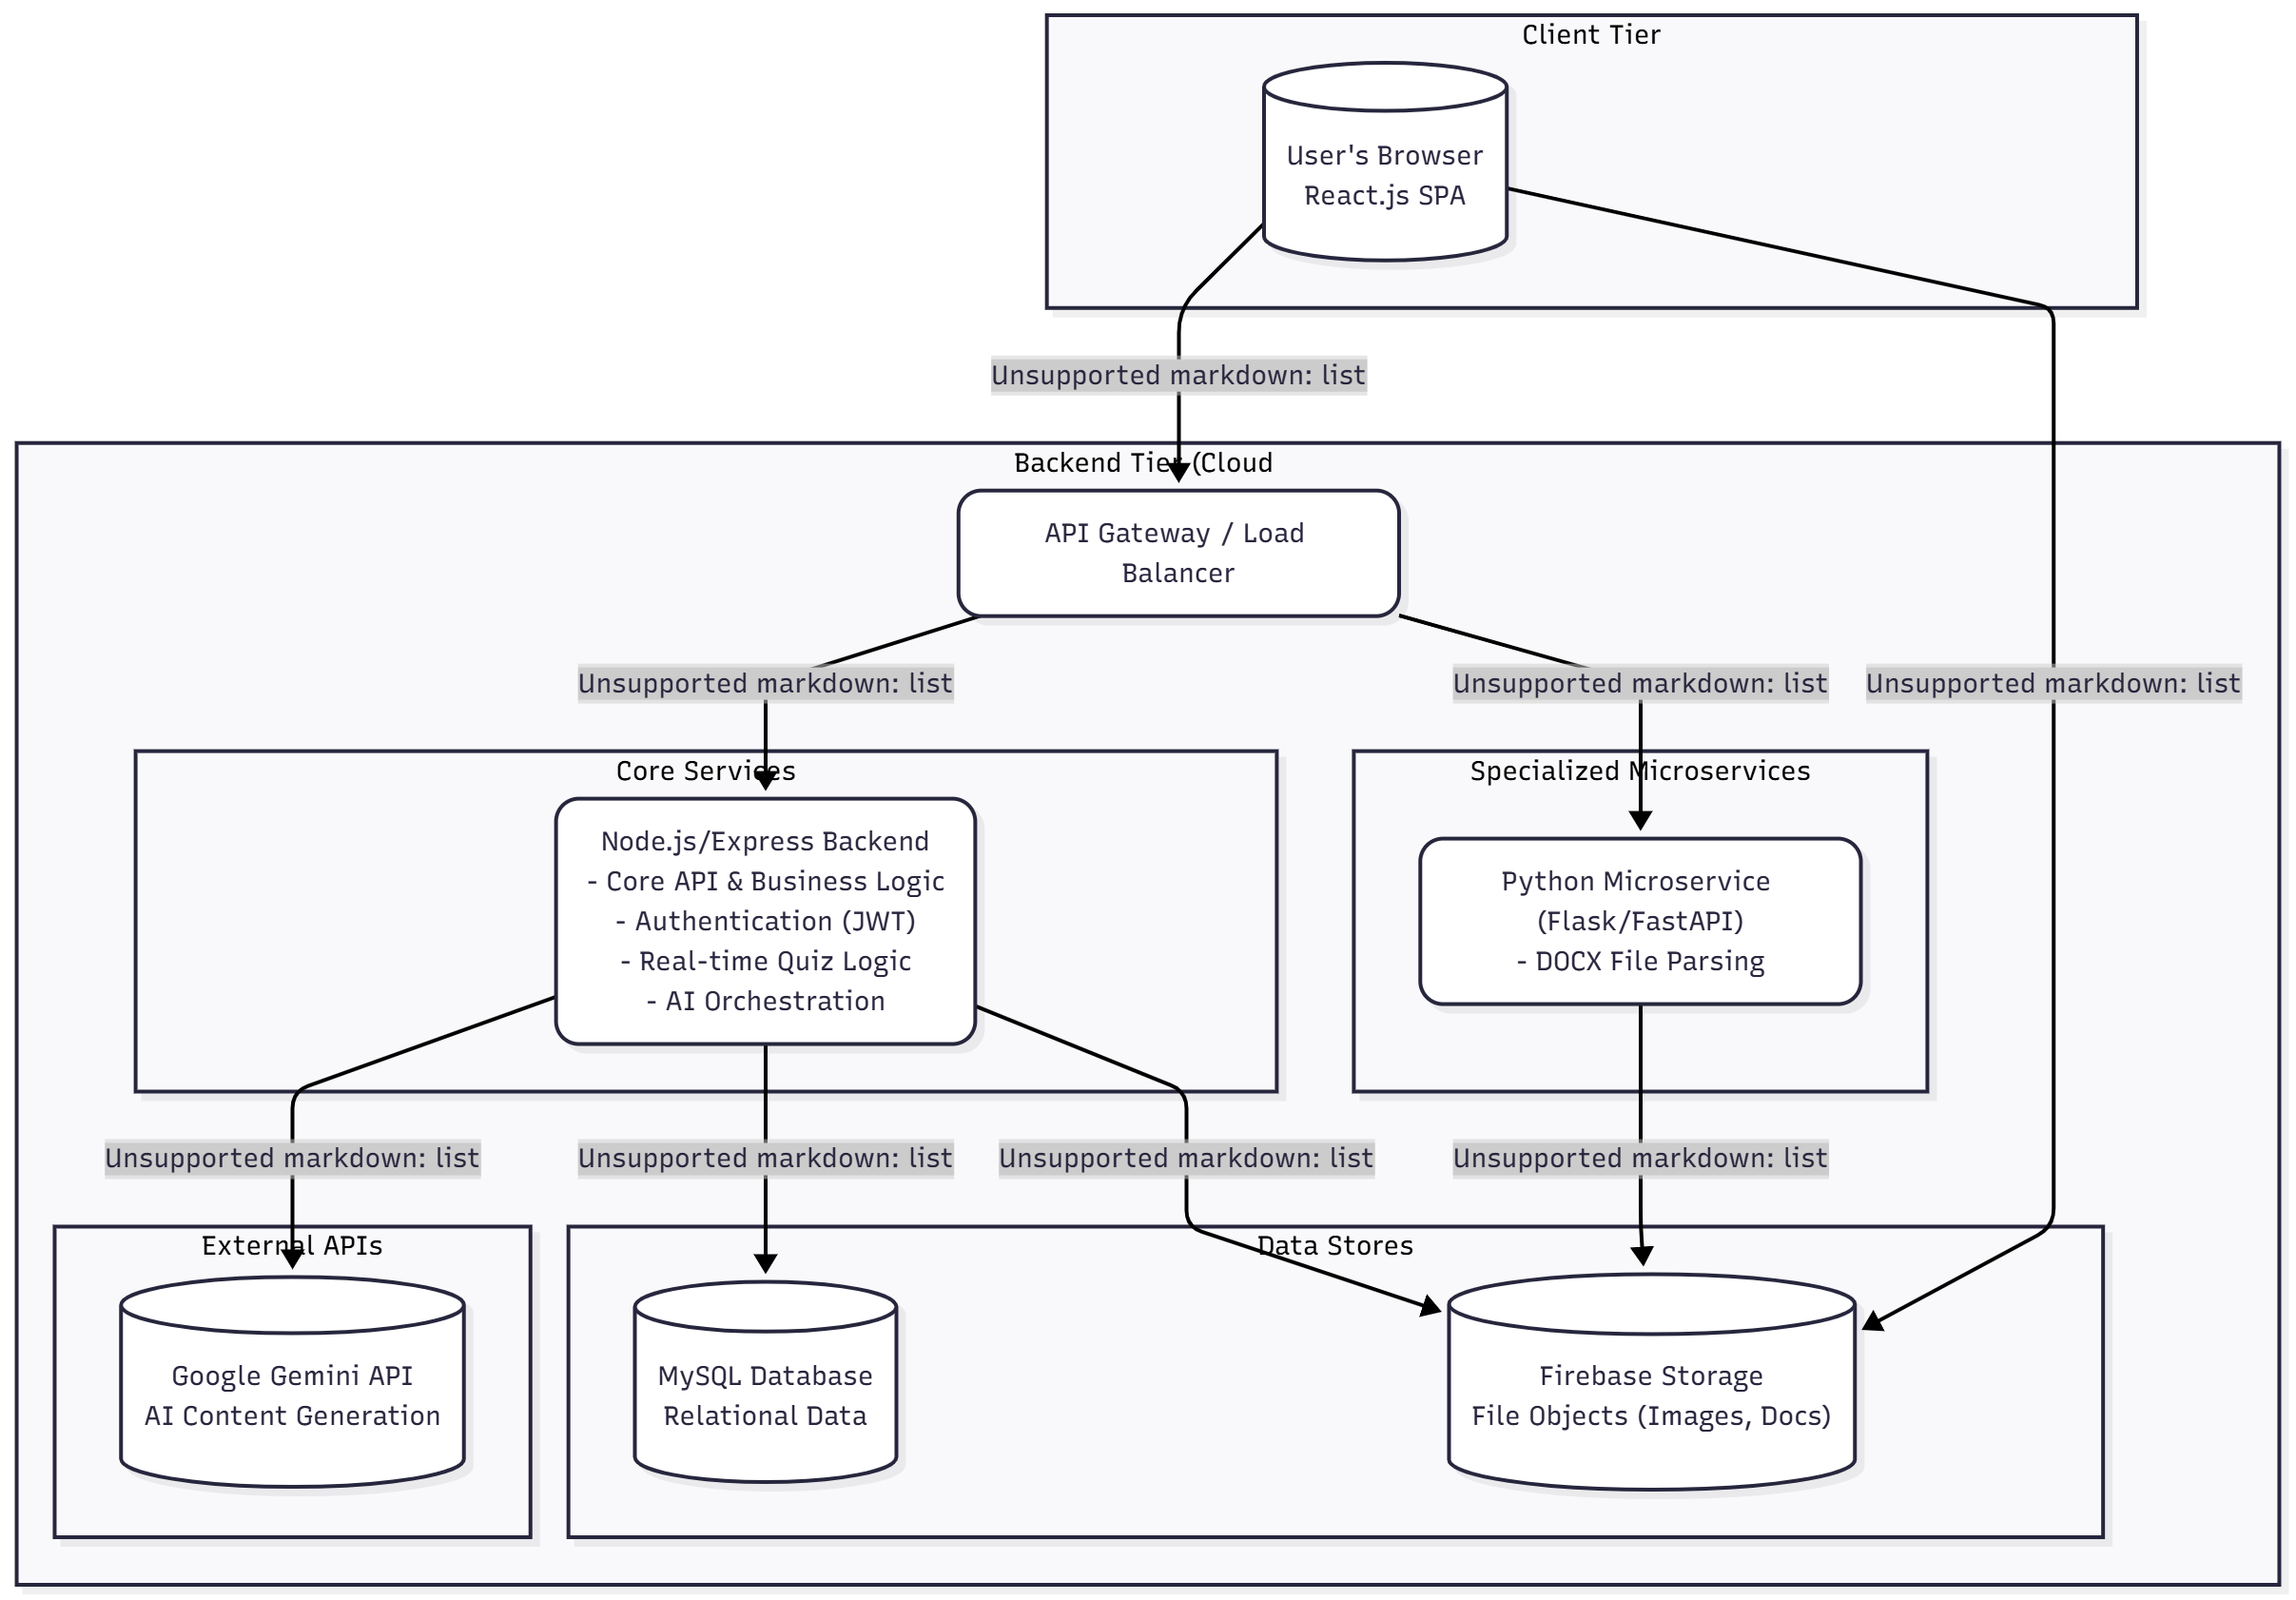
\includegraphics[width=\textwidth]{figures/system-architecture.png}
\caption{High-Level System Architecture of TEKUTOKO}
\label{fig:system-architecture}
\end{figure}

\paragraph{Architectural Flow:}
\begin{enumerate}
    \item The user interacts with the \textbf{React Single-Page Application (SPA)} in their browser.
    \item All API requests are sent via HTTPS to a central \textbf{API Gateway}, which acts as a reverse proxy and load balancer.
    \item Standard requests (user auth, room management, etc.) are routed to the \textbf{Node.js Backend}, the system's core. Requests specifically for DOCX file parsing are routed to the dedicated \textbf{Python Microservice}.
    \item The Node.js backend handles all business logic, interacting with the \textbf{MySQL Database} for persistent data storage.
    \item For file uploads, the Node.js backend generates a secure, short-lived "signed URL" from \textbf{Firebase Storage} and sends it to the client.
    \item The client uses this signed URL to upload the file directly to Firebase Storage, offloading bandwidth from the backend server.
    \item The backend orchestrates calls to the external \textbf{Google Gemini API} for question generation, handling prompt engineering and response parsing.
\end{enumerate}

\section{Component and Module Design}
\label{sec:arch-components}
\begin{itemize}
    \item \textbf{Frontend (React.js):} A modern SPA built with React 18 and styled with Tailwind CSS. It is responsible for rendering the entire user interface and managing client-side state using React Hooks and Context API. It communicates with the backend services via REST APIs.

    \item \textbf{Backend (Node.js/Express):} The central nervous system of the platform. Its responsibilities include providing RESTful API endpoints, managing JWT-based authentication, handling business logic for all core features, and orchestrating calls to other services.

    \item \textbf{Python Microservice (FastAPI/Flask):} A specialized service responsible for the complex task of processing `.docx` files. Its sole purpose is to accept a document, extract questions, options, and images, and convert them into a structured JSON format ready for serving. It orchestrates external command-line tools like \textbf{Pandoc} for document structure conversion and \textbf{ImageMagick} for image format transcoding (e.g., WMF/EMF to WebP). The processed output is stored in a static directory, served via HTTP, and its metadata is recorded in the database.

    \item \textbf{MySQL Database:} A relational database for all structured, persistent data. This includes user accounts, room configurations, questions, submissions, reward vouchers, and proctoring logs. The relational model ensures data integrity.

    \item \textbf{Firebase Storage:} A cloud-based object storage service used for all binary files, such as user avatars, room cover images, uploaded `.docx` documents, and files submitted by participants as answers.
\end{itemize}

\section{Database Design}
\label{sec:arch-database}

\subsection{Entity-Relationship Diagram (ERD)}
The relationships between the main entities in the system are illustrated in the ERD in Figure \ref{fig:erd-diagram}.

\begin{figure}[htbp]
\centering
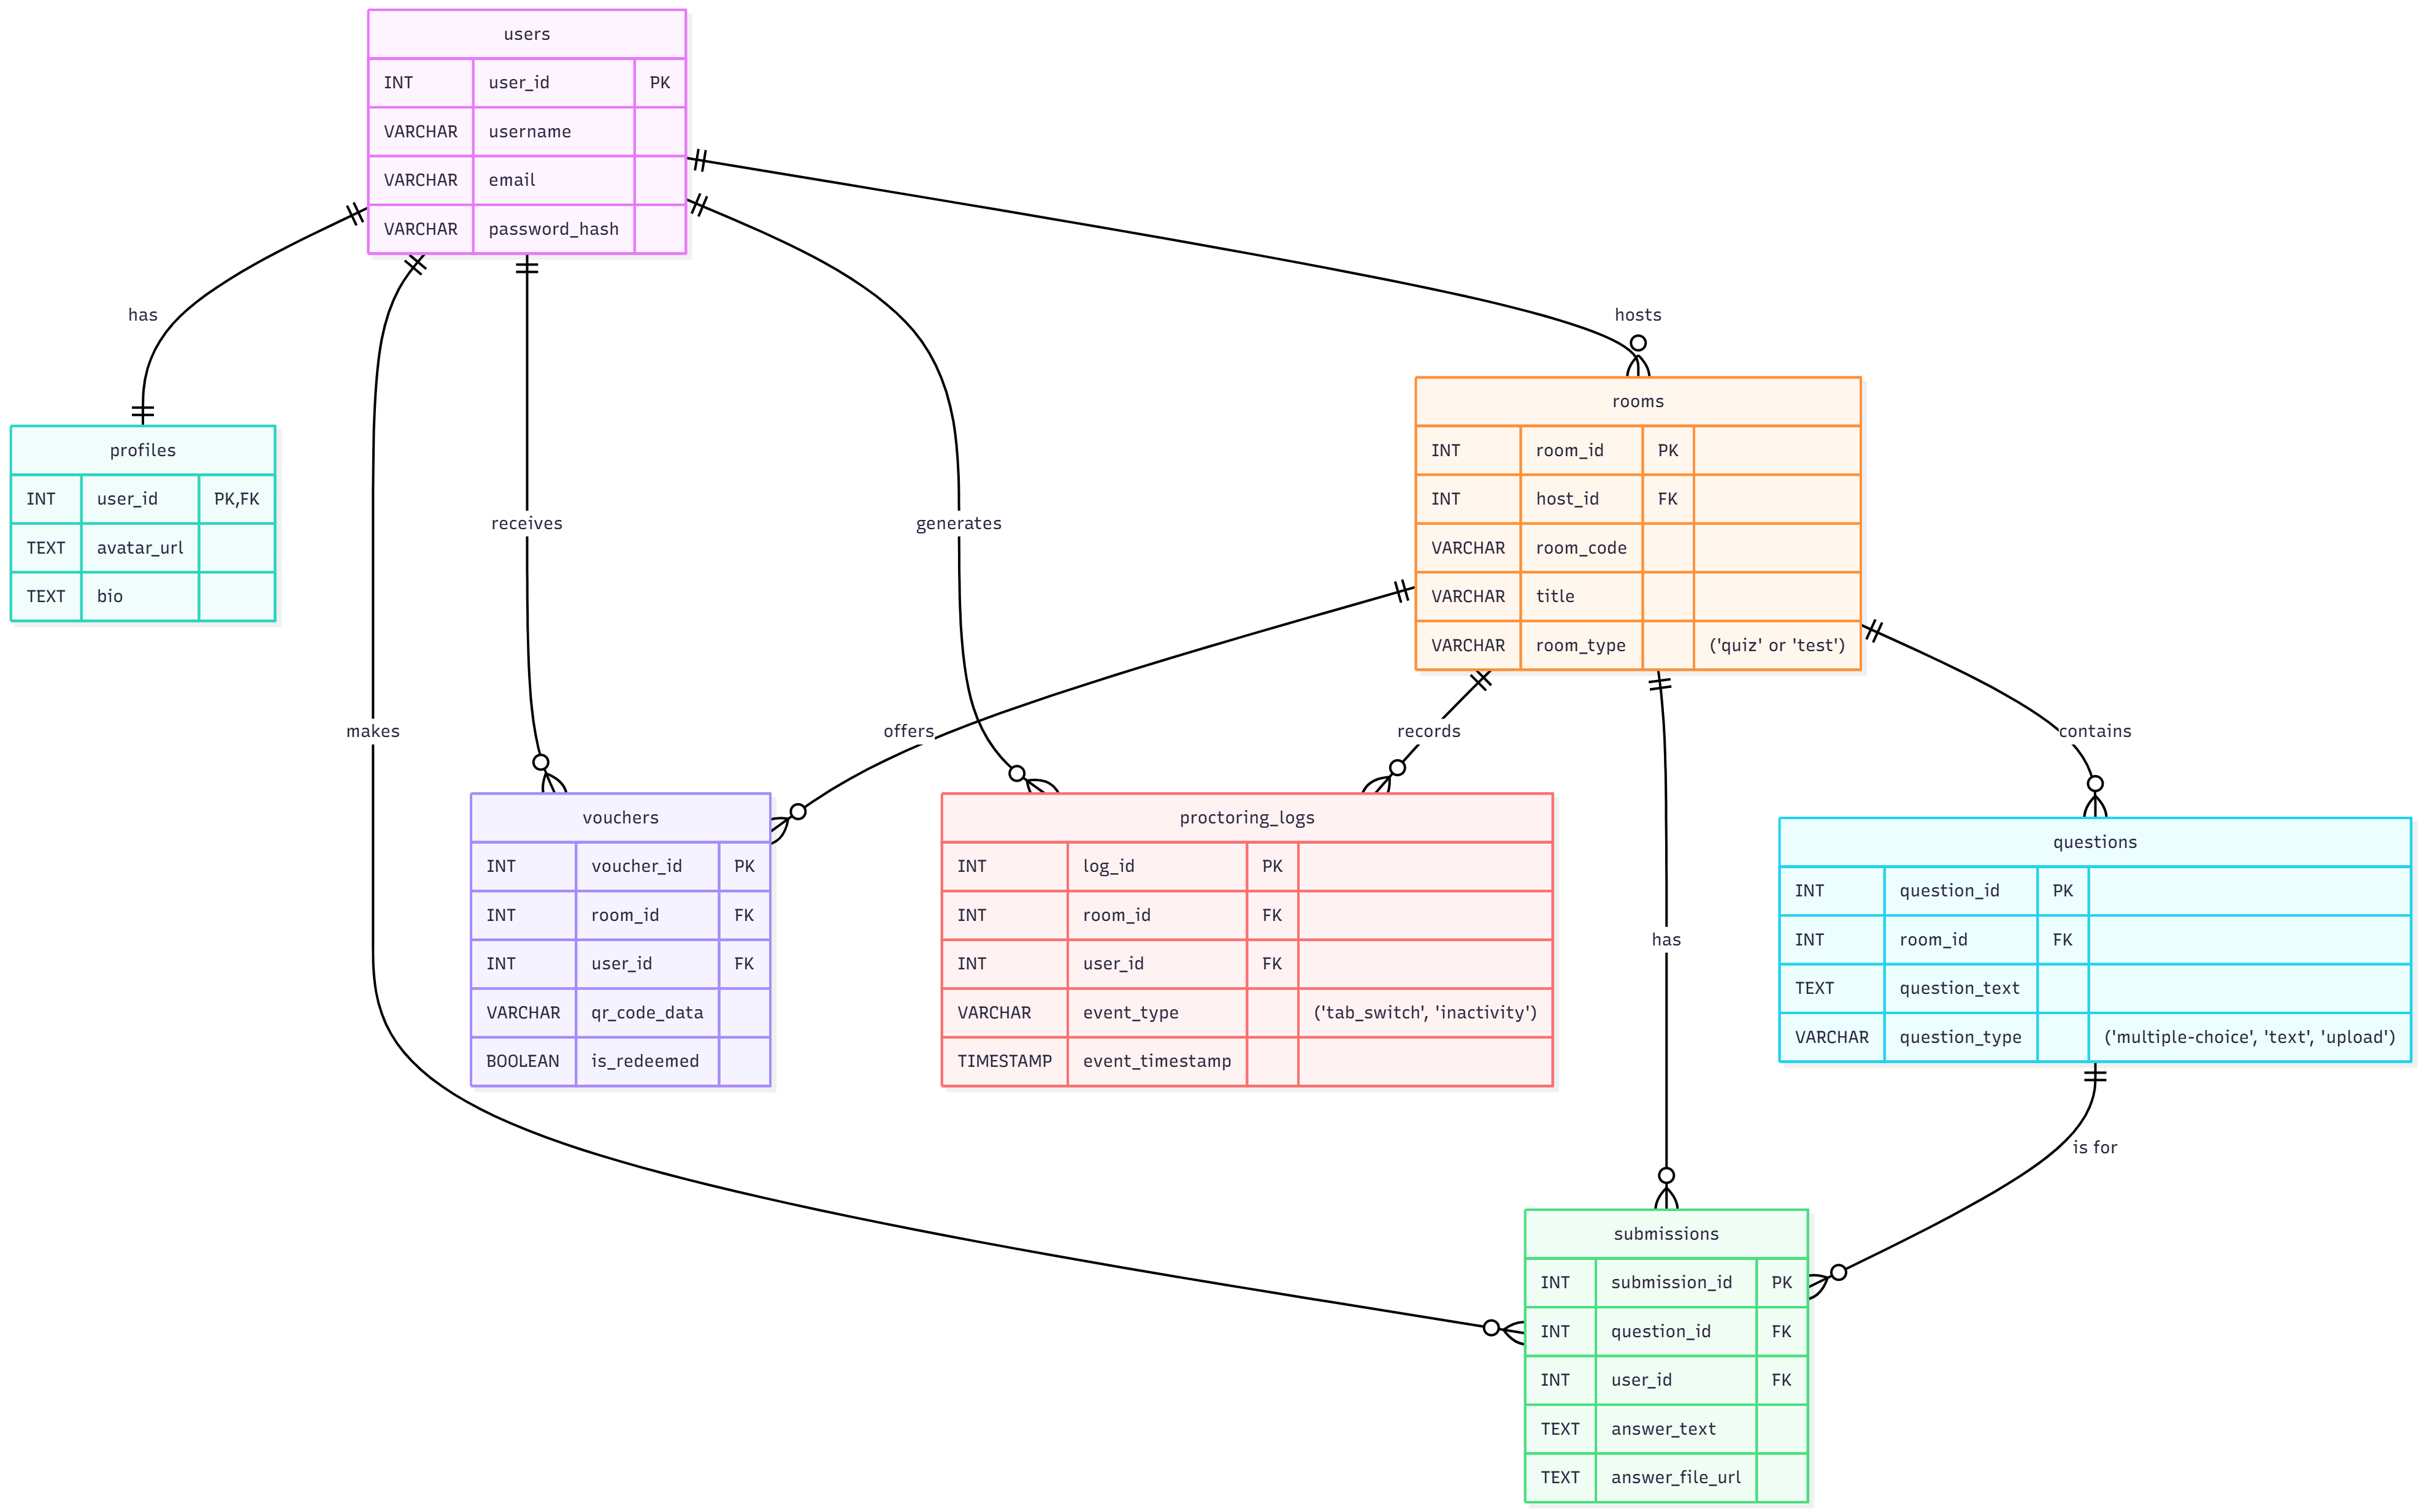
\includegraphics[width=\textwidth]{figures/erd-diagram.png}
\caption{Database Entity-Relationship Diagram (ERD)}
\label{fig:erd-diagram}
\end{figure}

\subsection{Detailed Table Schemas (Selected)}
Below are the SQL schemas for some of the key tables in the database.

\begin{lstlisting}[language=SQL, caption={SQL Schema for the `users` and `rooms` tables}]
-- Users table
CREATE TABLE `users` (
  `user_id` INT AUTO_INCREMENT PRIMARY KEY,
  `username` VARCHAR(50) NOT NULL UNIQUE,
  `email` VARCHAR(100) NOT NULL UNIQUE,
  `password_hash` VARCHAR(255) NOT NULL,
  `created_at` TIMESTAMP DEFAULT CURRENT_TIMESTAMP
);

-- Rooms table
CREATE TABLE `rooms` (
  `room_id` INT AUTO_INCREMENT PRIMARY KEY,
  `host_id` INT NOT NULL,
  `room_code` VARCHAR(8) NOT NULL UNIQUE,
  `title` VARCHAR(255) NOT NULL,
  `room_type` ENUM('quiz', 'test') NOT NULL,
  `gps_lat` DECIMAL(10, 8),
  `gps_lng` DECIMAL(11, 8),
  `created_at` TIMESTAMP DEFAULT CURRENT_TIMESTAMP,
  FOREIGN KEY (`host_id`) REFERENCES `users`(`user_id`) ON DELETE CASCADE
);
\end{lstlisting}

\begin{lstlisting}[language=SQL, caption={SQL Schema for the `proctoring_logs` and `vouchers` tables}]
-- Proctoring logs table
CREATE TABLE `proctoring_logs` (
  `log_id` INT AUTO_INCREMENT PRIMARY KEY,
  `room_id` INT NOT NULL,
  `user_id` INT NOT NULL,
  `event_type` ENUM('tab_switch', 'inactivity', 'paste_attempt') NOT NULL,
  `details` TEXT,
  `event_timestamp` TIMESTAMP DEFAULT CURRENT_TIMESTAMP,
  FOREIGN KEY (`room_id`) REFERENCES `rooms`(`room_id`) ON DELETE CASCADE,
  FOREIGN KEY (`user_id`) REFERENCES `users`(`user_id`) ON DELETE CASCADE
);

-- Vouchers table
CREATE TABLE `vouchers` (
  `voucher_id` INT AUTO_INCREMENT PRIMARY KEY,
  `room_id` INT NOT NULL,
  `user_id` INT NOT NULL,
  `qr_code_data` VARCHAR(255) NOT NULL UNIQUE,
  `reward_description` TEXT NOT NULL,
  `is_redeemed` BOOLEAN NOT NULL DEFAULT FALSE,
  `issued_at` TIMESTAMP DEFAULT CURRENT_TIMESTAMP,
  `redeemed_at` TIMESTAMP NULL,
  FOREIGN KEY (`room_id`) REFERENCES `rooms`(`room_id`),
  FOREIGN KEY (`user_id`) REFERENCES `users`(`user_id`)
);
\end{lstlisting}

\section{API Design and Specification}
\label{sec:arch-api}
The system exposes a RESTful API for communication between the frontend and backend. Endpoints are logically structured around resources, as shown in Table \ref{tab:api-endpoints}.

\begin{table}[htbp]
\centering
\caption{Key API Endpoint Specifications}
\label{tab:api-endpoints}
\resizebox{\textwidth}{!}{%
\begin{tabular}{l l p{6cm} l}
\toprule
\textbf{Method} & \textbf{Endpoint} & \textbf{Description} & \textbf{Auth Required} \\
\midrule
`POST` & `/auth/register` & Register a new user. & No \\
`POST` & `/auth/login` & Authenticate a user and return a JWT. & No \\
`POST` & `/api/rooms` & Create a new Quiz or Test Room. & Yes \\
`POST` & `/api/rooms/generate-ai` & Generate questions for a room using AI. & Yes \\
`POST` & `/api/v1/process-docx` & Upload a DOCX file for processing by the Python microservice. & Yes \\
`GET` & `/api/rooms/:roomCode` & Get public details for a specific room. & No \\
`POST` & `/api/rooms/:roomCode/submit` & Submit an answer to a question. & Yes \\
`POST` & `/api/rooms/:roomCode/log-proctor-event` & Log a suspicious event from a Test Room. & Yes \\
`GET` & `/api/discovery/nearby` & Find nearby rooms using GPS coordinates. & No \\
`POST` & `/api/vouchers/verify` & Verify a voucher via its QR code data. & Yes (Host) \\
\bottomrule
\end{tabular}%
}
\end{table}

\subsection{API Request/Response Example}
The following example shows the interaction for logging a proctoring event.

\paragraph{Request:} `POST /api/rooms/T5R8E2S1/log-proctor-event` (with participant's JWT)
\begin{lstlisting}[language=JSON]
{
  "eventType": "tab_switch",
  "details": "User switched away from the browser tab"
}
\end{lstlisting}

\paragraph{Response:} `200 OK`
\begin{lstlisting}[language=JSON]
{
  "status": "success",
  "message": "Proctoring event logged successfully."
}
\end{lstlisting}

\section{Security and Scalability Design}
\label{sec:arch-security-scalability}

\subsection{Authentication and Security}
\begin{itemize}
    \item \textbf{JWT-Based Authentication:} The system uses JSON Web Tokens for stateless authentication. After a successful login, the client receives an access token which is sent in the `Authorization` header of subsequent requests. The flow is visualized in Figure \ref{fig:jwt-flow}.
    \item \textbf{Password Security:} User passwords are never stored in plaintext. They are hashed using the `bcrypt` algorithm with a salt.
    \item \textbf{Voucher Security:} Each voucher is tied to a unique, cryptographically random string. The `is_redeemed` flag provides replay protection, ensuring a voucher can only be used once.
\end{itemize}

\begin{figure}[htbp]
\centering
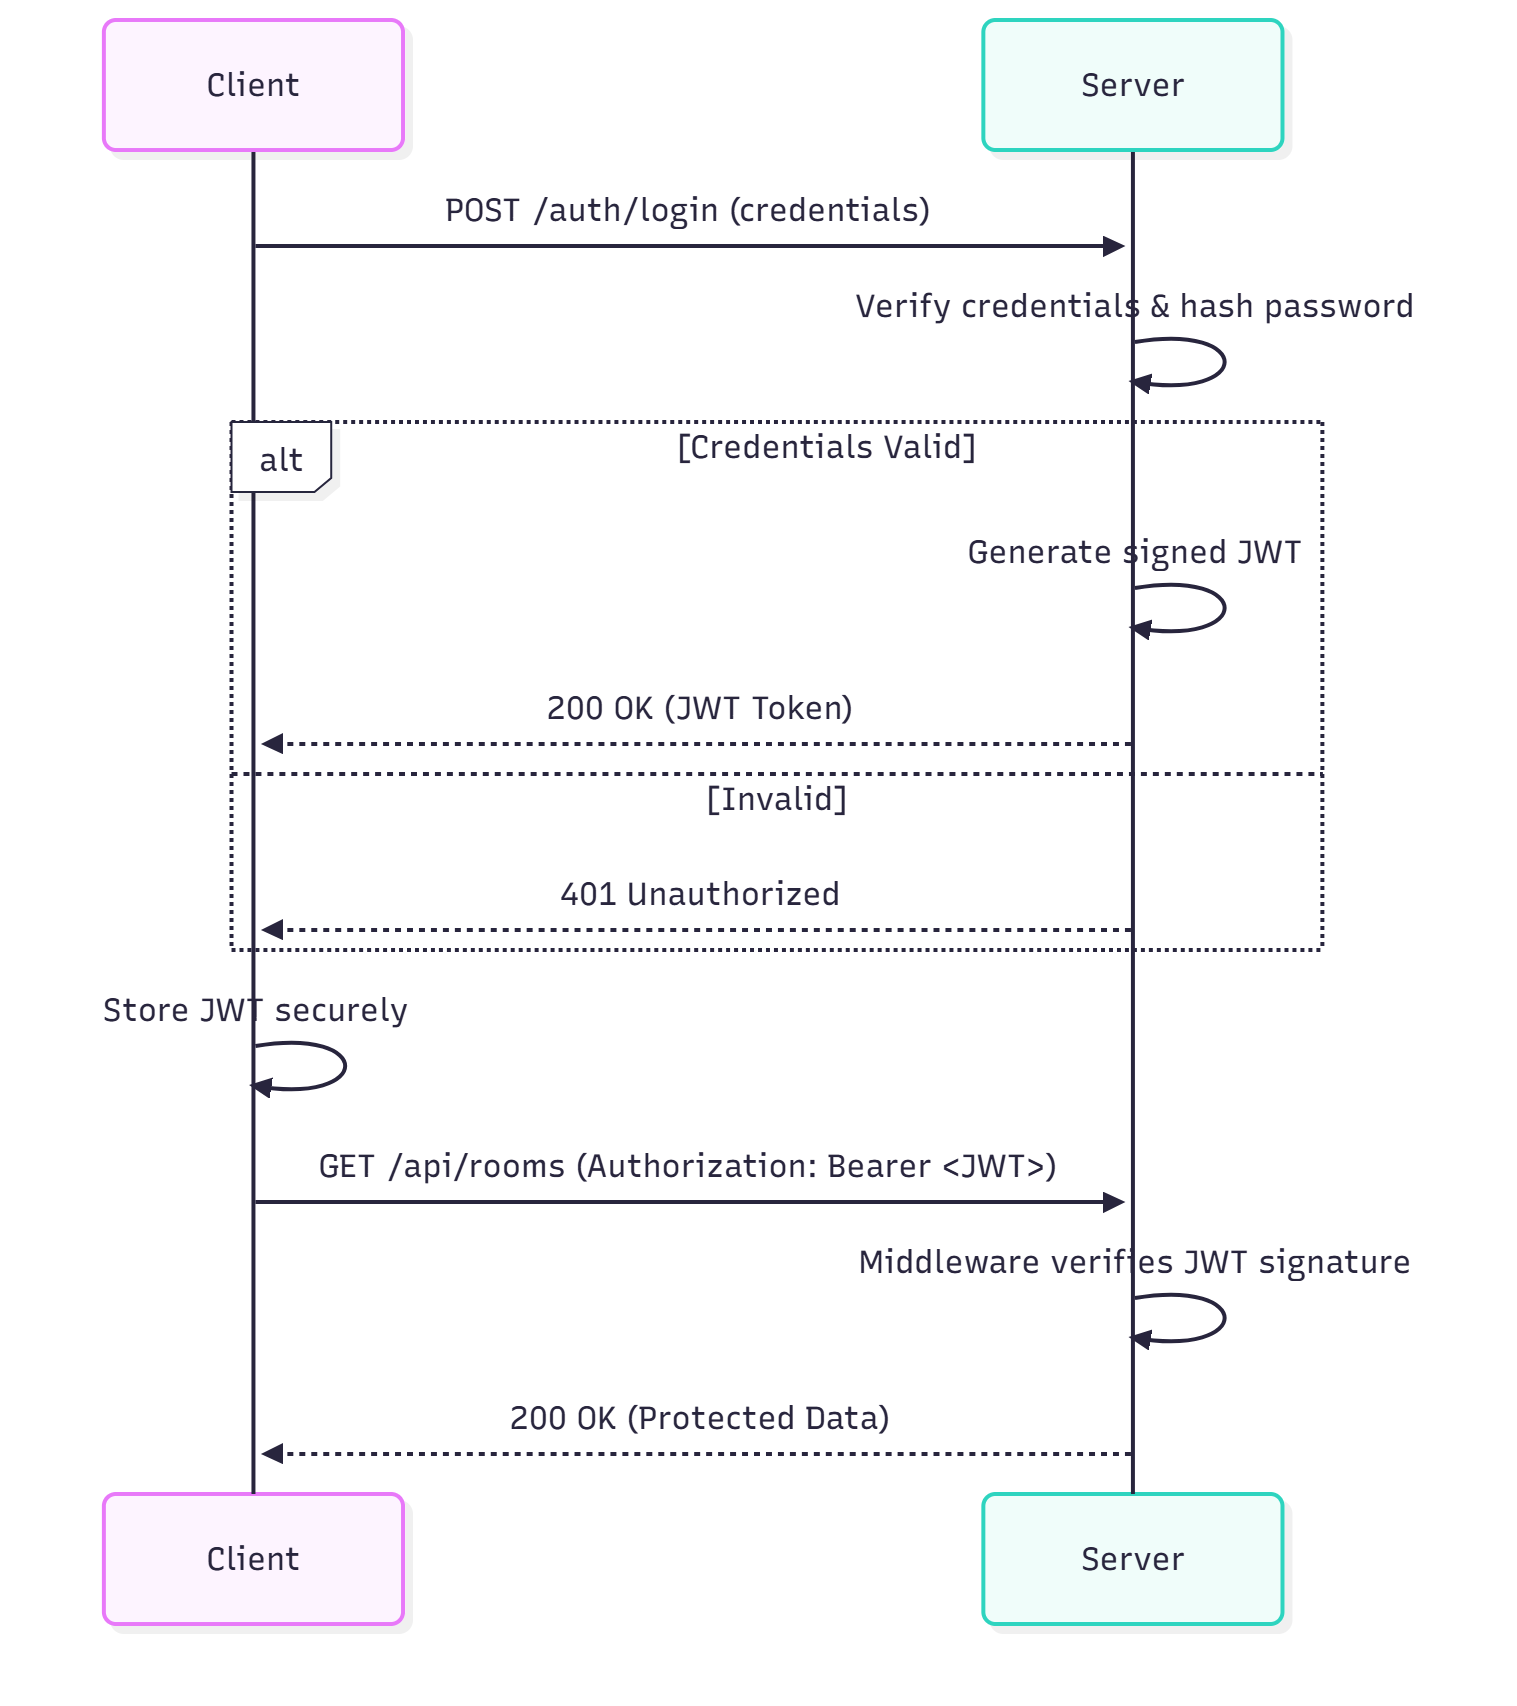
\includegraphics[width=0.7\textwidth]{figures/jwt-flow.png}
\caption{JWT-Based Authentication and Authorization Flow}
\label{fig:jwt-flow}
\end{figure}

\FloatBarrier
\subsection{Scalability}
\begin{itemize}
    \item \textbf{Stateless Backend:} The Node.js API server is designed to be completely stateless. It does not store any session-specific data in memory, allowing requests from a single user to be distributed across any available server instance.
    \item \textbf{Database Scaling:} The MySQL database can be scaled vertically (more powerful hardware) or horizontally using read replicas to distribute read-heavy query loads.
    \item \textbf{Independent Microservice Scaling:} If DOCX parsing becomes a bottleneck, the Python microservice can be scaled independently by deploying more instances, without affecting the performance of the core Node.js application. This is crucial as document and image processing are CPU-intensive tasks.
\end{itemize}